%%%%%%%%%%%%%%%%%%%%%%%%%%%%%%%%%%%%%%%%%%%%%%%%%%%%%%%%%%%%%%%%%%%%%%%%%%%%%%%%
% AMS Beamer series / Bologna FC / Template
% Andrea Omicini
% Alma Mater Studiorum - Università di Bologna
% mailto:andrea.omicini@unibo.it
%%%%%%%%%%%%%%%%%%%%%%%%%%%%%%%%%%%%%%%%%%%%%%%%%%%%%%%%%%%%%%%%%%%%%%%%%%%%%%%%
%\documentclass[handout]{beamer}\mode<handout>{\usetheme{default}}
%
\documentclass[presentation]{beamer}\mode<presentation>{\usetheme{AMSBolognaFC}}
%\documentclass[handout]{beamer}\mode<handout>{\usetheme{AMSBolognaFC}}
%%%%%%%%%%%%%%%%%%%%%%%%%%%%%%%%%%%%%%%%%%%%%%%%%%%%%%%%%%%%%%%%%%%%%%%%%%%%%%%%
\usepackage{mco-woa-kill-2022}
%%%%%%%%%%%%%%%%%%%%%%%%%%%%%%%%%%%%%%%%%%%%%%%%%%%%%%%%%%%%%%%%%%%%%%%%%%%%%%%%
\title[\killshort]
{\killshort: \killlong}
%
%\subtitle[AMS Series Templates]
%{AMS Series Templates}
%
\author[\sspeaker{Magnini et al.} ]
{\speaker{Matteo Magnini}$^{*}$ \and Giovanni Ciatto$^{*}$ \and Andrea Omicini$^{*}$}
%
\institute[DISI, Univ.\ Bologna]
{
    $^{*}$Dipartimento di Informatica -- Scienza e Ingegneria (DISI)\\\textsc{Alma Mater Studiorum} -- Universit{\`a} di Bologna
    \\
    \{\speaker{matteo.magnini}, giovanni.ciatto, andrea.omicini\}@unibo.it % emph the presenting author's email
}
%
\date[WOA 2022]{WOA 2022:\\Workshop “From Objects to Agents”\\September 1–2, 2022, Genova, Italy}
%
%%%%%%%%%%%%%%%%%%%%%%%%%%%%%%%%%%%%%%%%%%%%%%%%%%%%%%%%%%%%%%%%%%%%%%%%%%%%%%%%
\begin{document}
%%%%%%%%%%%%%%%%%%%%%%%%%%%%%%%%%%%%%%%%%%%%%%%%%%%%%%%%%%%%%%%%%%%%%%%%%%%%%%%%

%/////////
\frame{\titlepage}
%/////////

%%===============================================================================
%\section*{Outline}
%%===============================================================================
%
%%/////////
%\frame[c]{\tableofcontents[hideallsubsections]}
%%/////////

%===============================================================================
\section{Premises on \skilong}
%===============================================================================

%/////////
\begin{frame}[allowframebreaks]{\skilong}
    
    \begin{block}{Definition \ccite{surveyNeuroSymb,surveyXie,surveyCalegariCO20}}
        \skilong{} (\skishort) can be defined as:
        \begin{displayquote}\itshape
            any \emph{algorithmic} procedure affecting how \alert{sub-symbolic predictors} draw their inferences in such a way that predictions are either \emph{computed} as a function of, or made \emph{consistent} with, some \emph{given} \alert{symbolic knowledge}.
        \end{displayquote}
    \end{block}
    
    \framebreak
    
    \begin{block}{Symbolic knowledge}
        A symbolic representation consists of: \ccite{sub-symbolic-vs-symbolic}
        %
        \begin{enumerate}
            \item a set of symbols;
            \item\label{item:symbolic-combination} a set of grammatical rules governing the combining of symbols; 
            \item\label{item:symbolic-assignment} elementary symbols and any admissible combination of them can be assigned with meaning.
            %
            \begin{itemize}
                \item[$\Rightarrow$] Symbolic knowledge is both human and machine interpretable,
                \item first order logic (FOL) is an example of symbolic representation.
            \end{itemize}
        \end{enumerate}
    \end{block}
    
    \framebreak
    
    \begin{block}{Sub-symbolic predictors}
        \begin{itemize}
            \item deep neural networks (DNN);
            \begin{itemize}
                \item convolutional neural networks (CNN),
                \item recurrent neural networks (RNN);
            \end{itemize}
            \item kernel machines;
            \item basically everything that is sub-symbolic (models consisting of vectors, tensors, etc. of real numbers with no meaning for a human).
        \end{itemize}
    \end{block}
    
    \framebreak
    
    \begin{figure}
        \centering
        \subfloat{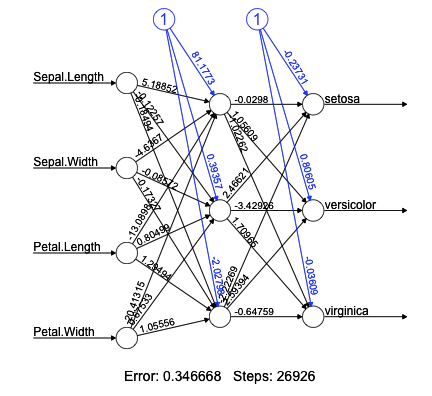
\includegraphics[width=0.4\textwidth]{figures/nn-iris}}
        %
        \qquad
        %
        \centering
        \subfloat{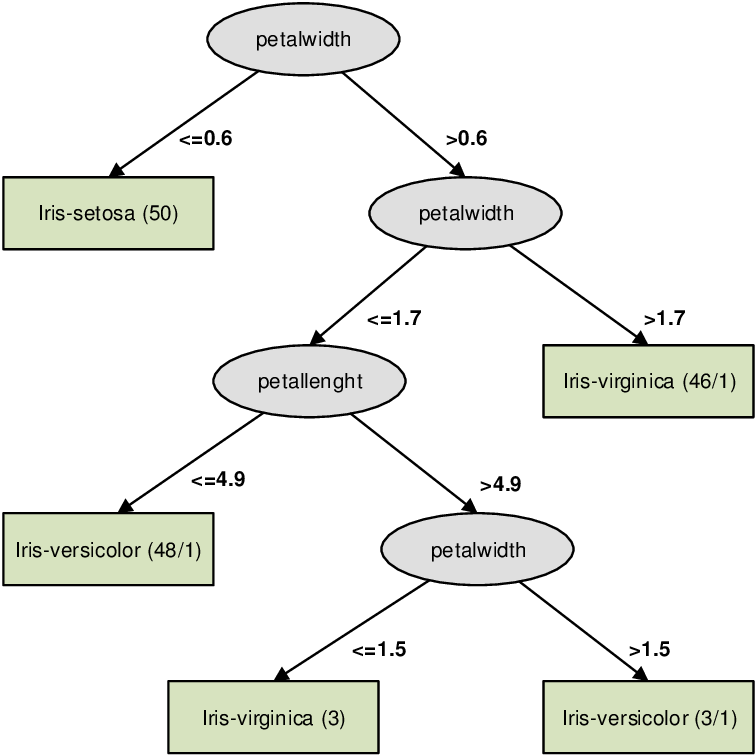
\includegraphics[width=0.4\textwidth]{figures/decision-tree-iris}}
    \end{figure}
    
    \framebreak
    
    Set of propositional logic rules built from the previous decision tree:
    
    \begin{equation*}
        \begin{aligned}
            \pred{iris}&(\var{SepalLenght}, \var{SepalWidth}, \var{PetalLenght}, \var{PetalWidth}, \const{setosa})\text{:-}\\
            &\var{PetalWidth} <= 0.6.\\
            \pred{iris}&(\var{SepalLenght}, \var{SepalWidth}, \var{PetalLenght}, \var{PetalWidth}, \const{versicolor}) \text{:-}\\
            &\var{PetalWidth} > 0.6, \var{PetalWidth} <= 1.7, \var{PetalLenght} <= 4.9.\\
            \pred{iris}&(\var{SepalLenght}, \var{SepalWidth}, \var{PetalLenght}, \var{PetalWidth}, \const{virginica}) \text{:-}\\
            &\var{PetalWidth} > 0.6, \var{PetalWidth} <= 1.5, \var{PetalLenght} > 4.9.\\
            \pred{iris}&(\var{SepalLenght}, \var{SepalWidth}, \var{PetalLenght}, \var{PetalWidth}, \const{versicolor}) \text{:-}\\
            &\var{PetalWidth} > 1.5, \var{PetalWidth} <= 1.7, \var{PetalLenght} > 4.9.\\
            \pred{iris}&(\var{SepalLenght}, \var{SepalWidth}, \var{PetalLenght}, \var{PetalWidth}, \const{virginica}) \text{:-}\\
            &\var{PetalWidth} > 1.7.\\
        \end{aligned}
    \end{equation*}

     \framebreak
    
    \begin{figure}
        \centering
        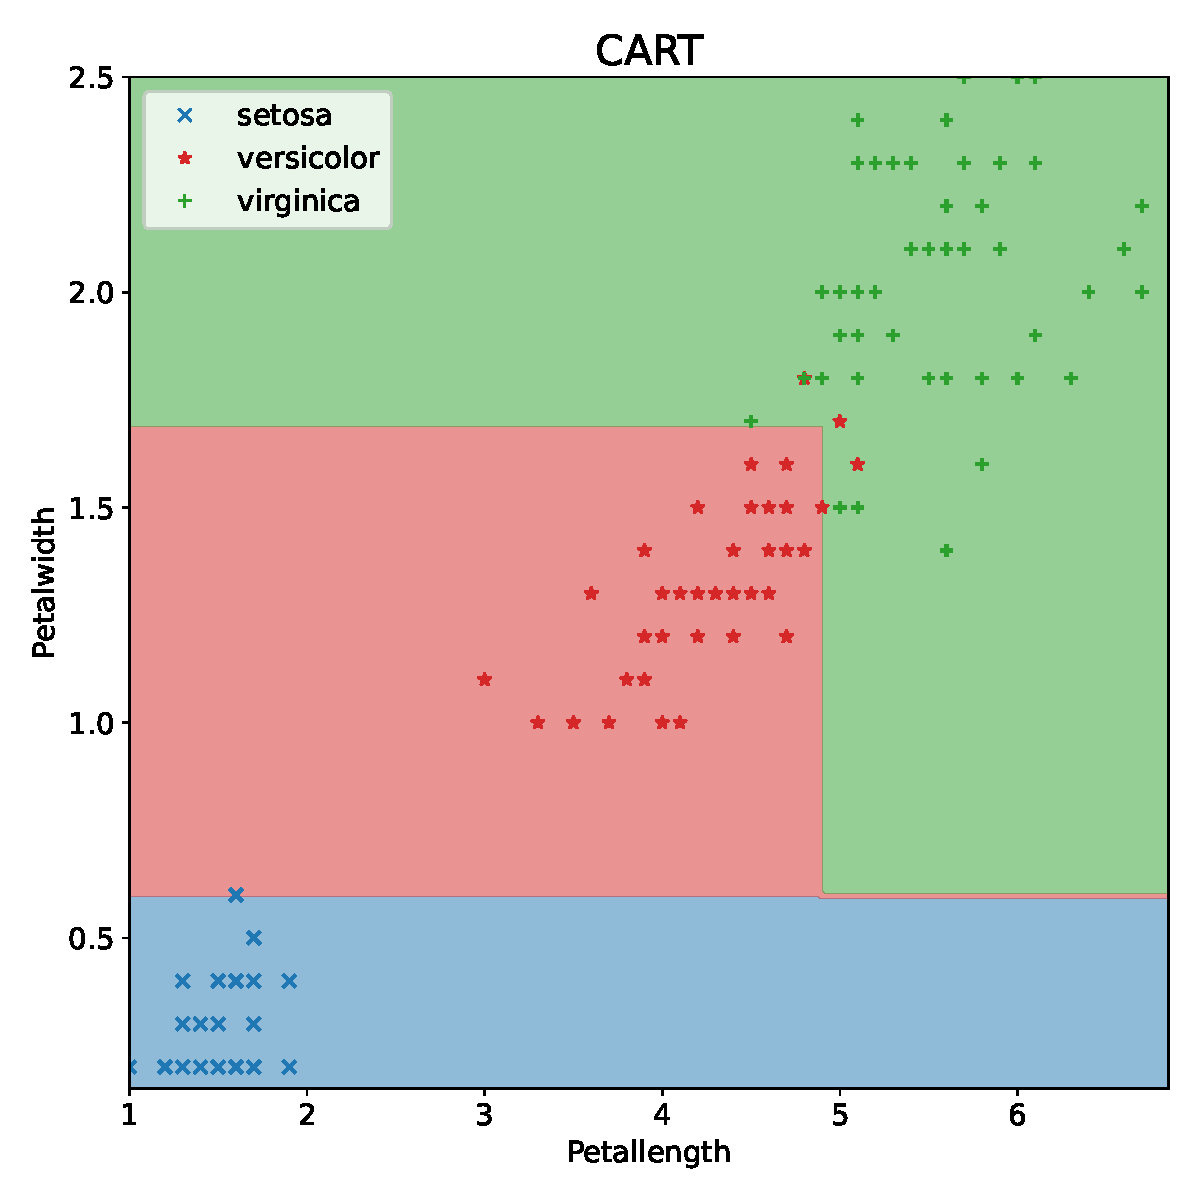
\includegraphics[width=0.5\textwidth]{figures/iris-plot.pdf}
    \end{figure}
    
    \framebreak
    
    \begin{block}{Why?}
        There are several benefits:
        %
        \begin{itemize}
            %
            \item prevent the predictor to become a black-box\alert{!};
            %
            \item reduce learning time;
            %
            \item reduce the data size needed for training;
            %
            \item improve predictor's accuracy;
            %
            \item build a predictor that behave as a logic engine.
        \end{itemize}
    \end{block}
    
    \framebreak
    
    Explainability can be achieved: \ccite{darpa2016-xai}
    %
    \begin{block}{Post-hoc explanation}
        \begin{itemize}
            \item applying an algorithm of symbolic knowledge extraction on a trained predictor;
            %
            \item output $\rightarrow$ logic rules that describe the predictor's behaviour.
            %
        \end{itemize}    
    \end{block}
    
    \begin{block}{By design}
        \begin{itemize}
            \item constraining the behaviour of predictors that are natively black-boxes with symbolic knowledge;
            %
            \item structuring the predictor's architecture with symbolic knowledge;
            %
            \item output $\rightarrow$ a predictor that does not violate the prior knowledge.
        \end{itemize}
    \end{block}
    
    %\end{frame}
    %/////////
    \framebreak
    %/////////
    %\begin{frame}[allowframebreaks]{Macro techniques}  
    
    \begin{block}{How?}
        There exist three major ways to perform knowledge injection on sub-symbolic predictors:
        %
        \begin{itemize}
            \item \alert{constraining}, a cost factor proportional to the violation of the knowledge is introduced during learning;
            \item \alert{structuring}, the architecture of the predictor is built in such a way to mimic the knowledge;
            \item \alert{embedding}, the symbolic knowledge is embedded into a tensor form and it is given in input as training data to the predictor.
        \end{itemize} 
    \end{block}
    
    \comment{
        \framebreak
        
        \begin{block}{Constraining}
            \begin{itemize}
                \item Knowledge cost factor is introduced in the loss function;
                %
                \item for NN the cost affects backpropagation \ccite{backpropagation} during training.
                %
                \begin{itemize}
                    \item[$\Rightarrow$] Predictor does not violate the prior knowledge (to a certain extent).
                \end{itemize} 
            \end{itemize}
        \end{block}
        
        \begin{figure}
            \centering
            \includegraphics[width=0.5\textwidth]{figures/ski-constraining}
        \end{figure}
        
        \framebreak
        
        \begin{figure}
            \centering
            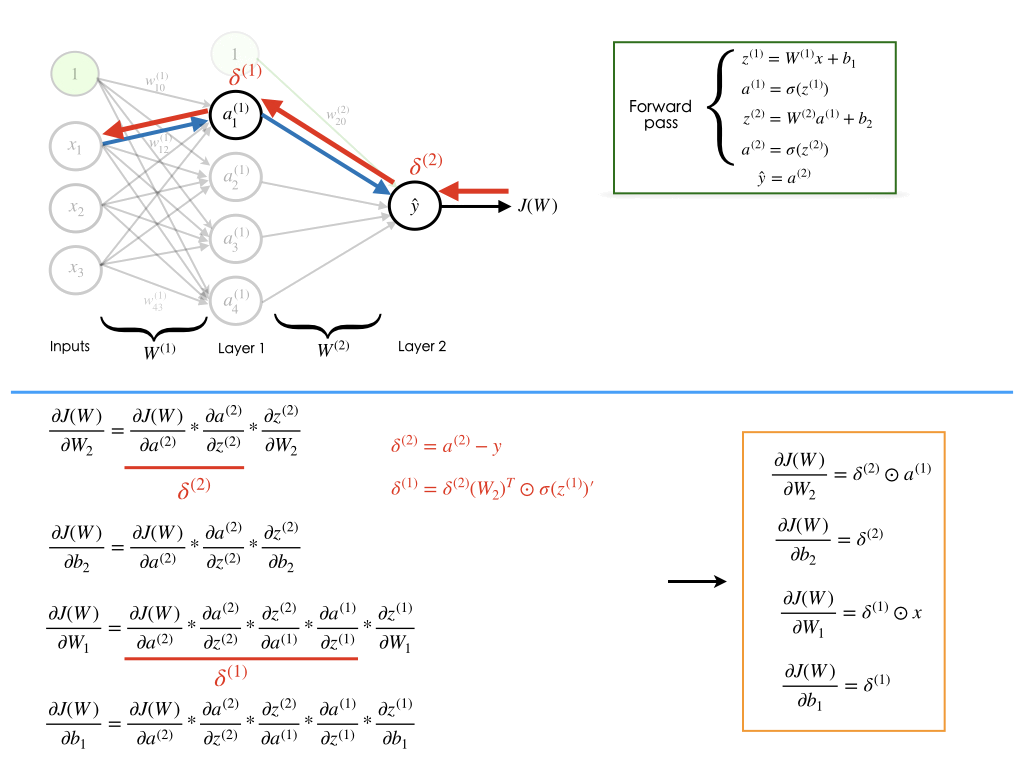
\includegraphics[width=0.8\textwidth]{figures/nn-backprop.png}
        \end{figure}
        
        \framebreak
        
        \begin{figure}
            \centering
            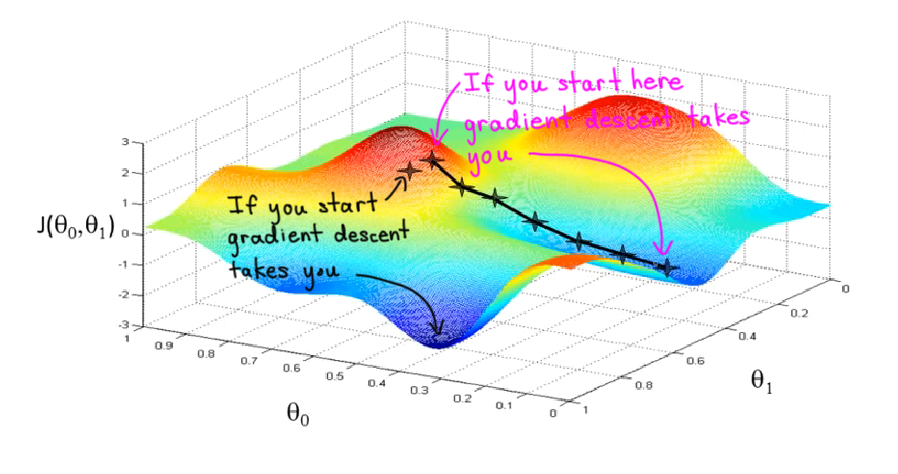
\includegraphics[width=0.8\textwidth]{figures/nn-gradient-descent.png}
        \end{figure}
        
        \framebreak
        
        \begin{block}{Structuring}
            \begin{itemize}
                \item Inner architecture is shaped to be able to ``mimic'' the knowledge;
                %
                \item for NN this means \emph{ad-hoc} layers.
                %
                \begin{itemize}
                    \item[$\Rightarrow$] Predictor directly exploits knowledge when needed.
                \end{itemize} 
            \end{itemize}
        \end{block}
        
        \begin{figure}
            \centering
            \includegraphics[width=0.6\textwidth]{figures/ski-structuring}
        \end{figure}
        
        \framebreak
        
        \begin{itemize}
            \item We need to define a mapping from crispy logic rules into fuzzy continuous interpretations;
            %
            \item then we need to map the interpretations into ad-hoc neurons/layers.
        \end{itemize}
        
        \begin{minipage}{0.45\textwidth}
            \begin{equation*}
                \begin{aligned}
                    \var{A}&\leftarrow\var{B}\wedge\var{C}\wedge\neg\var{D}.\\
                    \var{A}&\leftarrow\var{E}\wedge\var{F}.\\
                    \var{B}&\leftarrow\const{true}.\\
                \end{aligned}    
            \end{equation*}
        \end{minipage}
        %
        \begin{minipage}{0.45\textwidth}
            \begin{figure}
                \centering
                \includegraphics[height=0.5\textheight]{figures/structuring-example}
            \end{figure}
        \end{minipage}
        
        \framebreak
        
        \begin{block}{Embedding}
            
            \begin{itemize}
                \item Symbolic knowledge is embedded into a tensor form;
                %
                \item this is used as predictor's input data (alone or with a ``standard'' dataset).
                %
                \begin{itemize}
                    \item[$\Rightarrow$] Predictor's aim is manifold in most cases.
                \end{itemize} 
            \end{itemize}
            
        \end{block}
        
        \begin{figure}
            \centering
            \includegraphics[width=0.6\textwidth]{figures/ski-embedding}
        \end{figure}
        
        \framebreak
        %
        \begin{itemize}
            \item Knowledge graph embedding \ccite{kge-survey};
            %
            \item entities and relations are embedded into continuos vector spaces;
            %
            \item scoring function $f_{r}(h,t)$ defined on each fact $(h, r, t)$ to measure its plausibility;
        \end{itemize}
        %
        \begin{figure}
            \centering
            \includegraphics[width=0.8\textwidth]{figures/kge-space.png}
        \end{figure}
        
        \framebreak
        
        \begin{figure}
            \centering
            \includegraphics[width=0.8\textwidth]{figures/kge-nn-1.png}
        \end{figure}
        
        \begin{figure}
            \centering
            \includegraphics[width=0.8\textwidth]{figures/kge-nn-2.png}
        \end{figure}
    }
    
\end{frame}
%/////////

%===============================================================================
\section{\killshort{}: \killlong}
%===============================================================================

%/////////
\begin{frame}[allowframebreaks]{Algorithm}
    \begin{block}{\killshort: \killlong}
        %
        A general SKI algorithm that does not impose constrains on the sub-symbolic predictor to enrich, except being a neural network.
        %
        \begin{itemize}
            %
            \item aim $\rightarrow$ enrich;
            %
            \item predictor $\rightarrow$ neural network;
            %
            \item how $\rightarrow$ constraining;
            %
            \item logic $\rightarrow$ stratified Datalog with negation.
            %    
        \end{itemize}
    \end{block}
    %
    Public implementation on \psyki. \ccite{psyki}
    
    \framebreak
    
    \begin{figure}
        \centering
        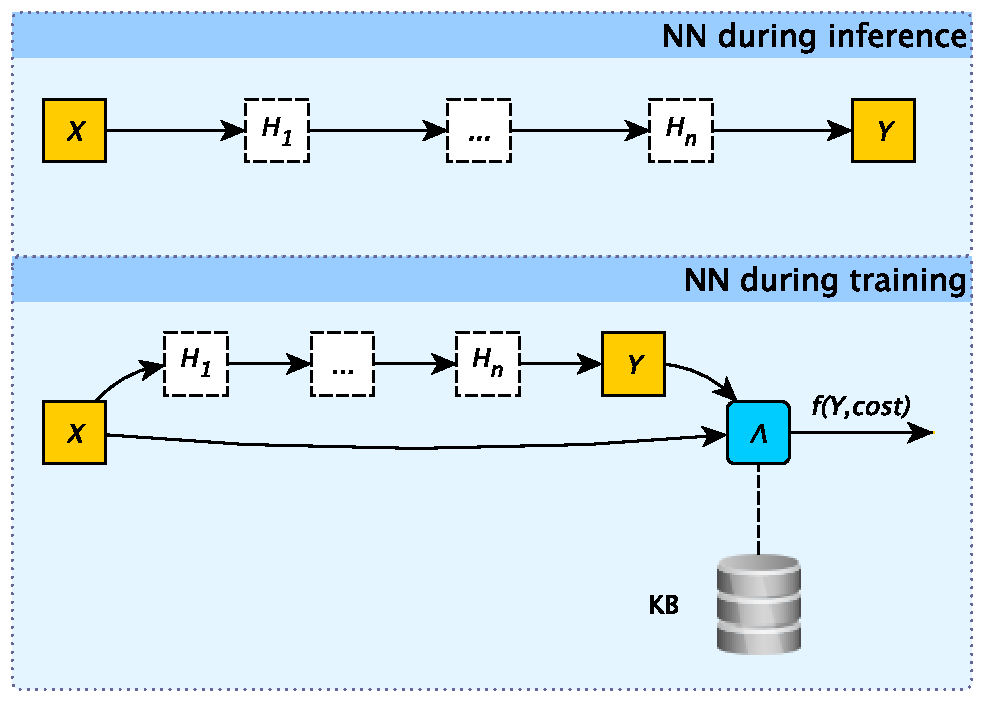
\includegraphics[width=0.8\textwidth]{figures/lambda-layer.pdf}
    \end{figure}
    
    \framebreak
    
    % !TeX spellcheck = en_GB
% !TeX root = ../ski-uai-2022.tex

\begin{table}%[!h]
    \centering
    \resizebox{\textwidth}{!}{%
        %
        %\caption{
            %Logic formul\ae's encoding into real-valued functions.
            %
            %There, $X$ is a logic variable, while $x$ is the corresponding real-valued variable, whereas is $\bar{X}$ a tuple of logic variables.
            %
            %Similarly, $\const{k}$ is a numeric constant, and $k$ is the corresponding real value, whereas $\const{k}_i$ is the constant denoting the $i^{th}$ class of a classification problem.
            %
            %Finally, $\text{expr}(\bar{X})$ is an arithmetic expression involving the variables in $\bar{X}$.
        %}
        %
        \label{tab:logic-formulae}
        %
        \begin{tabular}{l|r||cl|r}
            \textbf{Formula} & \textbf{C. interpretation} & & \textbf{Formula} & \textbf{C. interpretation}
            \\
            \hline\hline
            $\llbracket\neg \phi\rrbracket$ & $\eta(1 - \llbracket\phi\rrbracket)$ & & $\llbracket\phi \le \psi\rrbracket$  & $\eta(\llbracket\phi\rrbracket - \llbracket\psi\rrbracket)$
            \\
            $\llbracket\phi  \wedge \psi\rrbracket$ &  $\eta(max(\llbracket\phi\rrbracket, \llbracket\psi\rrbracket))$ & & $\llbracket \pred{class}(\bar{X}, \const{y}_i) \leftarrow \psi \rrbracket$ & $\llbracket \psi \rrbracket^{*}$
            \\
            $\llbracket\phi  \vee \psi\rrbracket$ & $\eta(min(\llbracket\phi\rrbracket, \llbracket\psi\rrbracket))$ & & $\llbracket \text{expr}(\bar{X}) \rrbracket$ & $\text{expr}(\llbracket\bar{X}\rrbracket)$
            \\
            $\llbracket\phi = \psi\rrbracket$ & $\eta(|\llbracket\phi\rrbracket-\llbracket\psi\rrbracket|)$ & & $\llbracket \mathtt{true} \rrbracket$ & $0$
            \\
            $\llbracket\phi \ne \psi\rrbracket$ & $\llbracket \neg ( \phi = \psi )\rrbracket$ & & $\llbracket \mathtt{false} \rrbracket$ & $1$
            \\
            $\llbracket\phi > \psi\rrbracket$  & $\eta(0.5 - \llbracket\phi\rrbracket + \llbracket\psi\rrbracket) $ & & $\llbracket X \rrbracket$ & $x$
            \\
            $\llbracket\phi \ge \psi\rrbracket$ & $\eta(\llbracket\psi\rrbracket - \llbracket\phi\rrbracket)$ & & $\llbracket \const{k} \rrbracket$ & $k$
            \\
            $\llbracket\phi < \psi\rrbracket$  &  $\eta(0.5 + \llbracket\phi\rrbracket - \llbracket\psi\rrbracket)$ & & $\llbracket \pred{p}(\bar{X}) \rrbracket^{**}$ & $\llbracket \psi_1 \vee \ldots \vee \psi_k \rrbracket$
            
        \end{tabular}
    }
    %
    \begin{center}\scriptsize
        $^{*}$ encodes the penalty for the $i^{th}$ neuron
        \\
        \smallskip
        $^{**}$ assuming predicate $p$ is defined by $k$ clauses of the form:
        \\
        $\pred{p}(\bar{X}) \leftarrow \psi_1,\ \ldots,\ \pred{p}(\bar{X}) \leftarrow \psi_k$
    \end{center}
\end{table}
    
    \framebreak
    
    \begin{equation*}
        \centering
        \begin{aligned}
            &Y' = f(Y, \pred{cost})\\
            &f = Y\ x\ (\textbf{1} + \pred{cost})\\
            &\pred{cost}(X,Y) = \eta(\pred{p}(X) - (\textbf{1} - Y))\quad\text{(because 0 means true)}\\
            \cline{1-2}
            X &= [5.0, 3.4, 1.5, 0.2]\quad (\const{setosa})\\
            Y &= [0.1, 0.9, 0]\quad (\const{setosa},\const{versicolor},\const{virginica})\\
            Y' &= [0.1, 0.9, 0]\ x\ (\textbf{1} + \pred{cost}([5.0, 3.4, 1.5, 0.2],[0.1, 0.9, 0]))\\
            \pred{cost} &= \eta(\pred{iris}([5.0, 3.4, 1.5, 0.2]) - [0.9, 0.1, 1])\\
            \pred{cost} &= \eta([0, 0.9, 0] - [0.9, 0.1, 1])\\
            \pred{cost} &= [0, 0.8, 0]\\
            Y' &= [0.1, 0.9, 0]\ x\ (\textbf{1} + [0, 0.8, 0])\\
            Y' &= [0.1, 1.62, 0]\\
        \end{aligned}
    \end{equation*}
    
    \framebreak
    
    \begin{equation*}
        \centering
        \begin{aligned}
            X &= [5.0, 3.4, 1.5, 0.2]\quad (\const{setosa})\\
            \pred{iris}&(\var{SepalLenght}, \var{SepalWidth}, \var{PetalLenght}, \var{PetalWidth}, \const{versicolor}) \text{:-}\\
            &\var{PetalWidth} > 0.6, \var{PetalWidth} <= 1.7, \var{PetalLenght} <= 4.9.\\
            \pred{iris}&(\const{5.0}, \const{3.4}, \const{1.5}, \const{0.2}, \const{versicolor}).\\
            &= (0.2 > 0.6) \vee (0.2 \le 1.7) \vee (1.5 \le 4.9)\\
            &= \eta(\pred{max}(\pred{max}(\eta(0.5 - 0.2 + 0.6), \eta(0.2 - 1.7)), \eta(1.5 - 4.9))))\\
            &= \eta(\pred{max}(\pred{max}(0.9, 0), 0)))\\
            &= 0.9
        \end{aligned}
    \end{equation*}

    \framebreak
    
    \begin{figure}
        \centering
        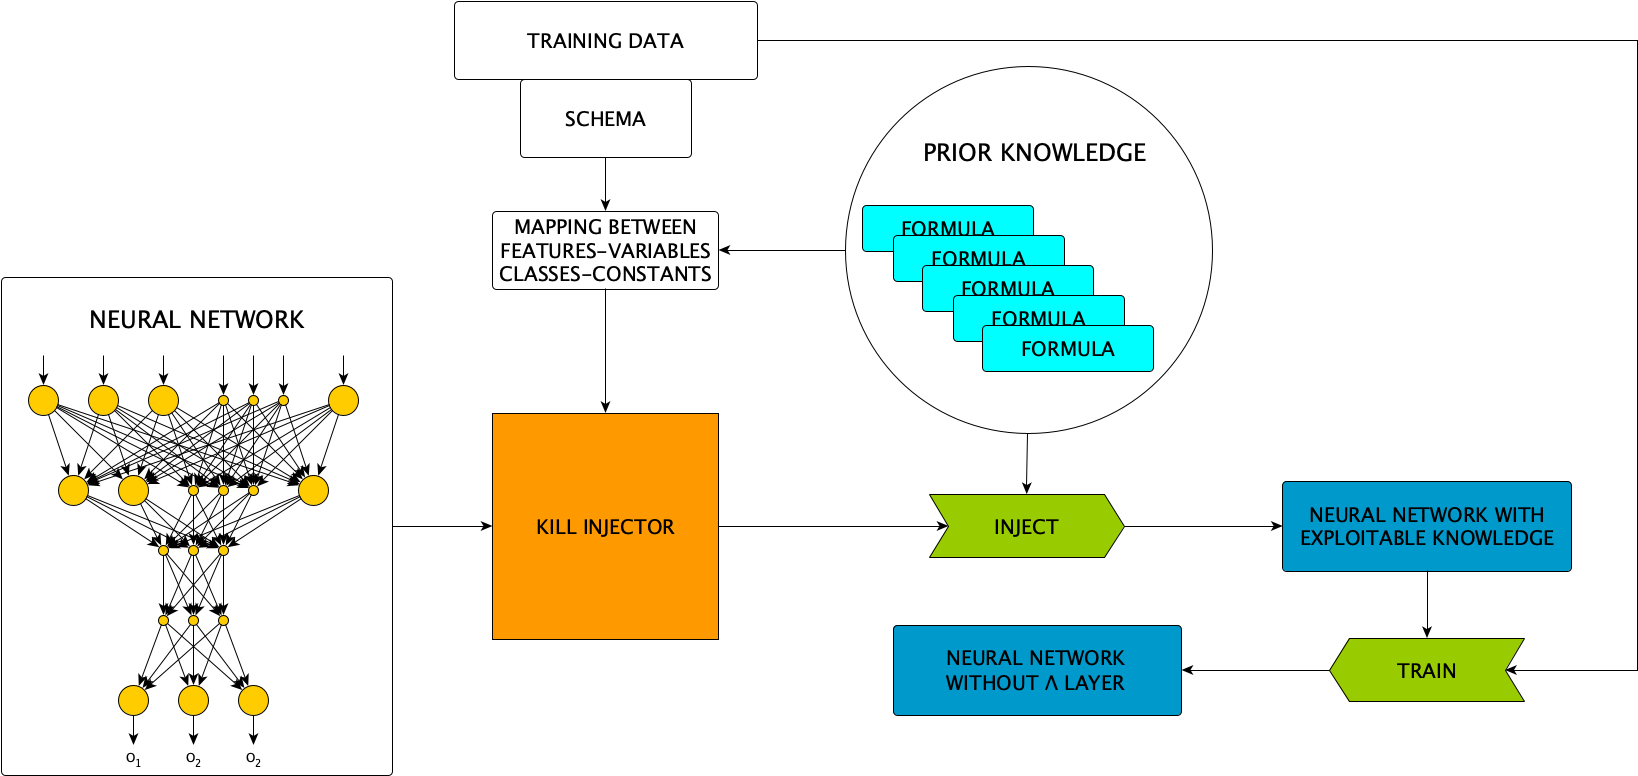
\includegraphics[width=0.9\textwidth]{figures/kill.png}
    \end{figure}
    
\end{frame}

%===============================================================================
\section{Case study}
%===============================================================================

%/////////
\begin{frame}[allowframebreaks]{Case study}
    Empty page
\end{frame}

%===============================================================================
\section*{}
%===============================================================================

%/////////
\frame{\titlepage}
%/////////

%===============================================================================
\section*{\refname}
%===============================================================================

%%%%
\setbeamertemplate{page number in head/foot}{}
%/////////
\begin{frame}[c,allowframebreaks,noframenumbering]{\refname}
    %\begin{frame}[t,allowframebreaks,noframenumbering]{\refname}
    %	\tiny
    \scriptsize
    %	\footnotesize
    \bibliographystyle{apalike-AMS}
    \bibliography{mco-woa-kill-2022}
\end{frame}
%/////////

%%%%%%%%%%%%%%%%%%%%%%%%%%%%%%%%%%%%%%%%%%%%%%%%%%%%%%%%%%%%%%%%%%%%%%%%%%%%%%%%
\end{document}
%%%%%%%%%%%%%%%%%%%%%%%%%%%%%%%%%%%%%%%%%%%%%%%%%%%%%%%%%%%%%%%%%%%%%%%%%%%%%%%%
